Figure \ref{fig:the proposed approach} shows the proposed approach to the ASL translator. The main approach to developing a translation from American SLA to other SLA is to build the best image recognition model that recognizes each English alphabet from the sign language with high accuracy. Instead of learning from scratch, Transfer learning with pre-trained models, which were already trained on a large benchmark image dataset, can save a lot of computation cost and help the performance. Kera applications provide a wide range of pre-trained models for deep learning such as VGG, ResNet, Xception, etc \cite{keras}. All the available pre-trained models will be applied into the first run training with the partial dataset to find out the Top 5 models with the highest accuracy of prediction. The top 5 models are further optimized and trained with all the training data to determine the best ASL recognition model. In the last phase, the results of prediction are mapping with Turkish ASL images.

\begin{figure}[h]
    \centering
    \caption{The proposed approach for the sign language translator}
	\label{fig:the proposed approach}
    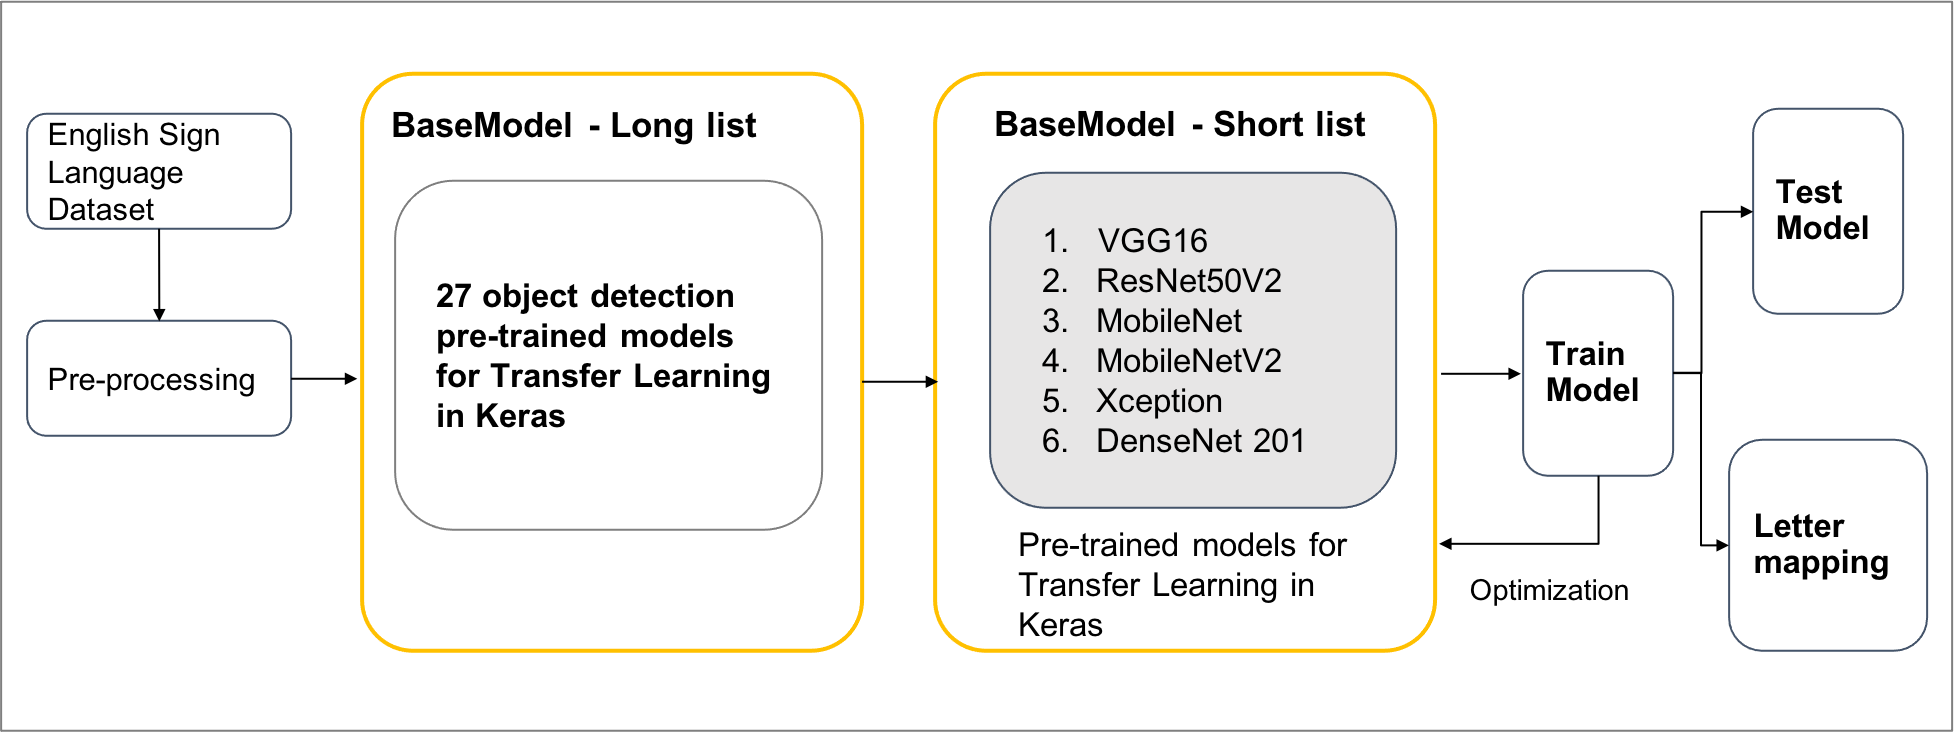
\includegraphics[width=\linewidth]{figures/The approach}
\end{figure}


\subsection{Dataset}
The American ASL dataset is collected from Kaggle. The dataset contains 87,000 images with 26 Englich alphabets and 3 extra signs, which are delete, space, and nothing. All the images are equally distributed to the 29 signs. In other words, each sign has 4,300 images. The whole dataset is split into training and test dataset. Training dataset is 80\% of the data, and the rest data belongs to the test dataset. 


\subsection{Image preprocessing}

\subsection{Transfer learning models}
One of the main benefits of using transfer learning is to make use of previously trained models and save computational cost (CC) for basic tasks like the removal of background. It may also be used when the training data is sparse. For the detection of American SLA we may use (to a degree) any pre-trained model for object detection on our dataset of American SLA signs even if they are limited in count and quality, as they only make the last layer of our final model.

To determine, whether a model may be suitable for our application, we use all of the models and its variants available in Keras\cite{keras}, as shown in Table~\ref{tab:keras_models}. The \textit{Avg. Top-5 Accuracy} in the table refers to the average accuracy of all variants combined.
\begin{table}[th]
    \caption{Keras Applications}
    \label{tab:keras_models}
    \centering
    \begin{tabular}{@{}lrcl@{}}
    \toprule
    Name         & \multicolumn{1}{l}{\begin{tabular}[c]{@{}l@{}}Avg. Top-5\\ Accuracy\end{tabular}} & \multicolumn{1}{l}{Total} & \begin{tabular}[c]{@{}l@{}}Variants\\ (*=Model)\end{tabular}                         \\ \midrule
    Xception     & 0.945                                                                             & 1                         & *                                                                                    \\
    VGG          & 0.901                                                                             & 2                         & *16, *19                                                                             \\
    ResNet       & 0.931                                                                             & 6                         & \begin{tabular}[c]{@{}l@{}}*50, *101, *152,\\  *50V2, *101V2,\\  *152V2\end{tabular} \\
    Inception    & 0.945                                                                             & 2                         & *V3, *ResNetV2                                                                       \\
    MobileNet    & 0.898                                                                             & 2                         & *, *V2                                                                               \\
    DenseNet     & 0.930                                                                             & 3                         & *121, *169, *201                                                                     \\
    NASNet       & 0.940                                                                             & 2                         & *Mobile, *Large                                                                      \\
    EfficientNet & -                                                                                 & 8                         & \begin{tabular}[c]{@{}l@{}}*B0, *B1, *B2,\\  *B3, *B4, *B5,\\  *B6, *B7\end{tabular} \\ \bottomrule
    \end{tabular}
\end{table}

In order to determine, which of the above stated models we will further evaluate and possibly optimize, we train each of the Keras models in an experimental setup. The experimental training is defined by:
\begin{enumerate}
    \item Training with 5\% of the dataset (~4.300 images, equally distributed to the 29 targets), with a 80/20 Train-Test-Split
    \item 10 Epochs of Training
    \item No Early Stopping
\end{enumerate}

The results will focus on two key indicators: accuracy on our dataset and training time.

\subsubsection{VGG16}

\subsubsection{ResNet50V2}

\subsubsection{MobileNet}

\subsubsection{MobileNetV2}

\subsubsection{DenseNet 201}

\subsubsection{Xception}